\documentclass[10pt]{scrartcl}

\usepackage[a4paper, left=20mm, right=20mm, top=30mm, bottom=40mm]{geometry}

% UTF8 character set
\usepackage[utf8]{inputenc}

% T1 encoding
\usepackage[T1]{fontenc}
\usepackage{ngerman}
\usepackage{graphicx, xcolor}

% Write correct
\usepackage{siunitx}

\usepackage{epstopdf}

\usepackage{amsmath}

% use sans serif fonts
% \renewcommand{\familydefault}{\sfdefault}

% headings, footer
\usepackage{fancyhdr}

% last page indicator
\usepackage{lastpage}

% formatting captions
\usepackage[center,format=hang,nooneline,labelsep=quad,font={small},labelfont=bf,figurewithin=none]{caption}
\captionsetup[figure]{name=Figure}

% typewriter for URLs
\usepackage[pdfpagelabels=true,plainpages=false]{hyperref}
\renewcommand{\refname}{References}
\begin{document}

% Define lengths.
\setlength{\textheight}{21cm}
\setlength{\parindent}{0cm}
\setlength{\headheight}{1.75cm}
\setlength{\headsep}{1cm}
\setlength{\footskip}{1.5cm}

\renewcommand{\headrulewidth}{0pt} 
\renewcommand{\footrulewidth}{0pt} 
%\renewcommand{\figurename}{Abbildung} 

\pagestyle{fancy}
\lhead{\vspace*{-0.6cm}\hspace*{-1cm}
\includegraphics[scale=0.5]{logo.png}}
\rhead{Human Computer Interaction\\Wintersemester 2020/21\\ \today}
\lfoot{}
\cfoot{\thepage\ -- \pageref{LastPage}}
%\rfoot{\hspace{2cm}\includegraphics[scale=1]{images/logo-slogan}}

\begin{flushright}
{Group G606\\ Exercise Sheet -1}
\end{flushright}
\section{Usability} 
\subsection{Name the six goals in which usability is usually broken down into with example for each.}
	
	\begin{enumerate}
		\item \textbf{Effective to use:} Is it doing the function that it is supposed to do accurately and completely? Can we obtain quality results that are standard for a device/interface of this nature?\\
	\emph{Ex - Wired earphones, they allow the user to perform the task in the right way (play, stop, skip the music) with good quality results.} 
		\item  \textbf{Efficient to use:} Once that user is comfortable with using the product, can the user accomplish his tasks with minimal time and energy? Is the interaction productive and economical?
		\emph{Ex - Word Processors such as Word/Pages - At first the features are overwhelming. But with every interaction, you realize the UI is intuitive.}
		
		\item\textbf{Safe to use: }How error-prone is the system, and if so how easily can we recover and go back to the original state that and as such retrieve our information? Are there any privacy/safety concerns?
		\emph{Ex - A digital payment service rollbacks the entire transaction in case of fault connection failure during the operation.}
		
		\item \textbf{Have good utility:} Does the system offer a flexible range of required and additional functions that helps in achieving of the task that it is supposed to smooth and devoid of errors. 
		\emph{Ex- A Microwave oven has a range of different heating/convection/time limits buttons that allows the user flexibility to warm and cook in different ways.}
		
		\item \textbf{Easy to learn :} Is the system’s operations and ways/function to perform such operations easily learnable to a novice or infrequent user? \emph{Ex- Operating Gmail - All Functionality is laid clearly and it maintains consistency with other mail clients.}
		
		\item \textbf{Easy to remember:} How involved are the steps to use a product/system? How many steps should the user remember to interact/use the product?
		\emph{Ex: On/Off buttons on most devices are prominent and marked/colored in Red or Green.}
				
	\end{enumerate}
	
\subsection{State how the design of Xbox Wireless Controller fulfills/does not fulfill the six usability goals.}

\begin{enumerate}
	\item \textbf{Effective to use :} Yes, the wireless controller fulfills the basic function of allowing the user to control the characters in the games through the use of button or the pad to move and perform action on the screen.
	
	\item\textbf{Efficient to use :} The wireless controller once charged can last up to 30 hours, providing an incredible way to sustain productivity. It also supports wired connection and replaceable batteries.
	
	\item \textbf{Safe to use  :} The wireless controller is robust, in that, any kind of error induced by the user has ramifications limited to the gaming environment (the character might die/lose a point).
	
	\item \textbf{Have a good utility :} The wireless controller supports a variety of functions such as compatibility with a wide range of devices and seamless pairing with multiple devices.
	
 \item \textbf{Easy to learn :} The wireless controller has a good geometric design with colorful buttons that allows the user to explore a variety of combinations to get the hang of using the device and the user can easily learn the button positions.
	
	\item \textbf{Easy to remember : } The buttons on the wireless controller, unfortunately are not readily relatable to any physical design, making it difficult for the user to remember the function of all the 12 buttons in different games. This is evident from an excerpt presented in the caption of Figure \ref{fig:xbox}.
	
\end{enumerate}


\begin{figure}
	\centering
	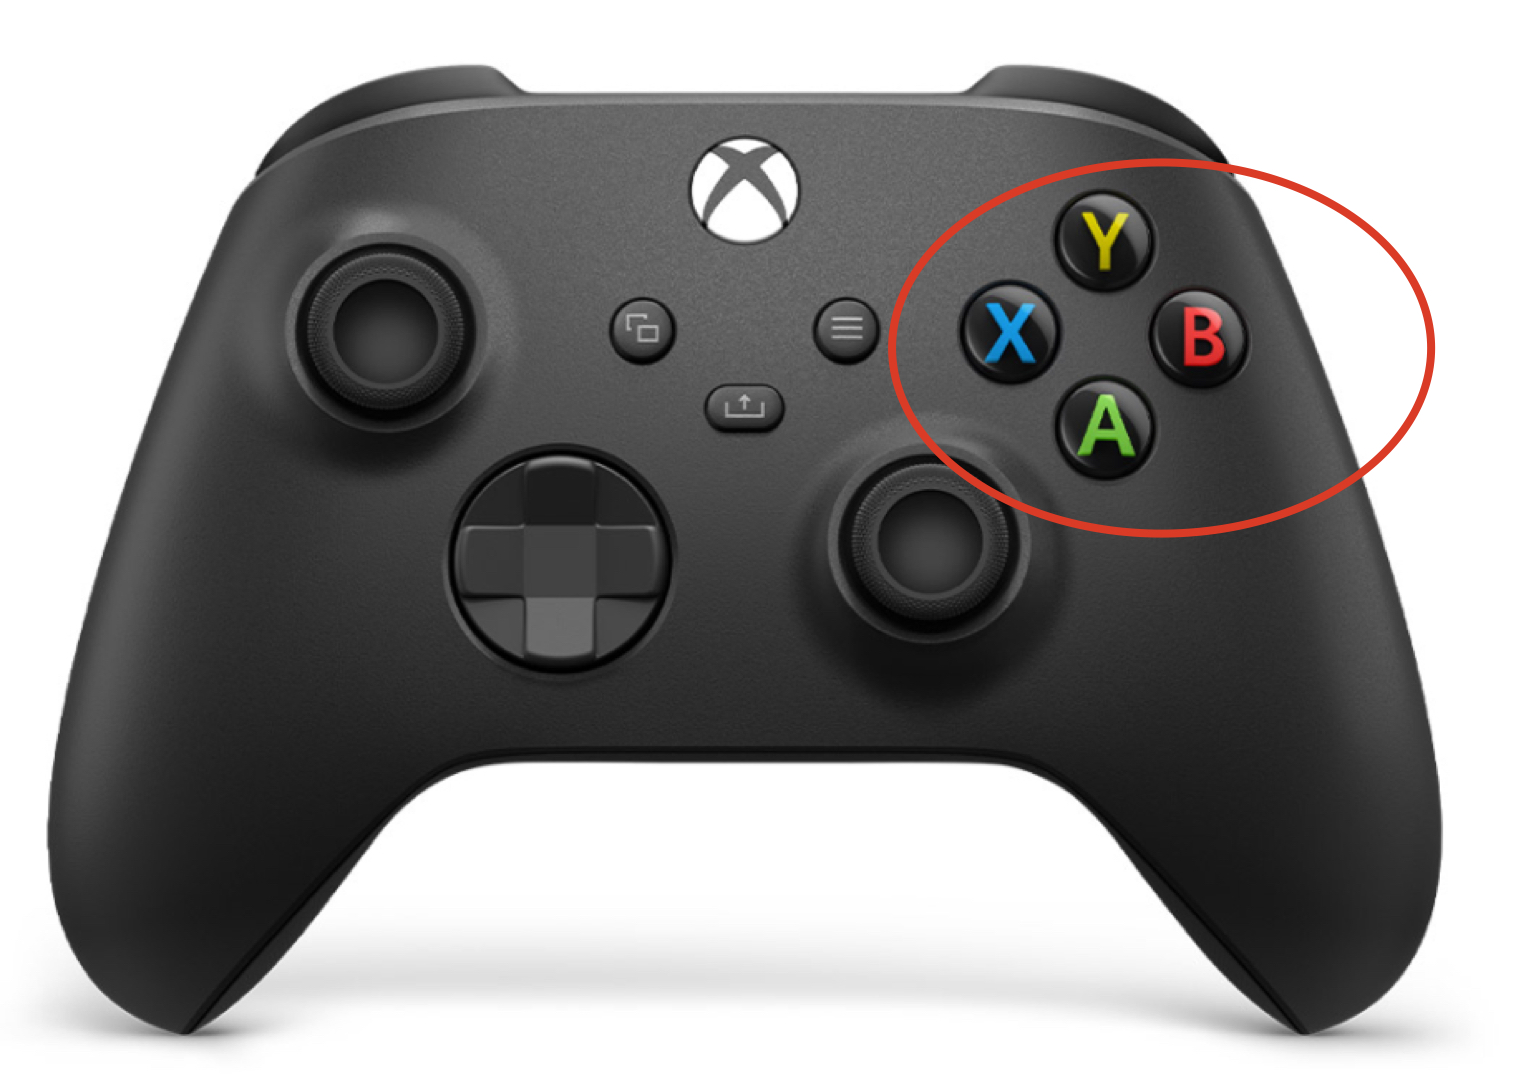
\includegraphics[width=0.2\linewidth]{xbox}
	\caption{``In North America and Europe, games commonly use X to confirm (the role of A) and O to cancel (the role of B.) In Japan, however, the O symbol is commonly associated with maru (right) while X is identified with batsu (wrong.) Therefore the roles are reversed, O confirms and X cancels. While the controls of most games are localized with this in mind, games such as Final Fantasy VII and Metal Gear Solid were left with their original mapping to the general confusion of Western players." - Credits : \href{http://gangles.ca/2008/09/16/a-brief-history-of-a-b/}{Buttons}. }
	\label{fig:xbox}
\end{figure}


\section{Interaction Modes }

\begin{enumerate}
	\item \textbf{You would like to pay for your parking ticket before leaving the parking garage in your car. (Do also consider the fact that some people might suffer from disabilities.)}
	
	Solution - Parking ticket vending machine that can be interacted via physical buttons and voice. The buttons also support braille. Mode of Interaction - Instructive and Manipulation.
	
	\item \textbf{You are walking in a foreign town using a pedestrian navigation system.}
	Solution - Pedestrian navigation system can be interacted with physical touch manipulation and also has a voice component. Mode of Interaction - Conversing and Manipulating.
	
	\item \textbf{You would like to follow a recipe for baking a cake for your friend’s birthday.}
	Solution - A system that shows you a permanent list of the ingredients and customize the portion number with a video tutorial that shows all steps that you can re-watch and play/stop when you want. Have to perform an audio description of the steps too. Mode of Interaction - Exploring and Manipulating.
	
	\item \textbf{You need to find a store in a mall using a public display}
	Solution - To find a store in a mall using an interactive touch screen display that allows you to select from a list the show that you want to reach. This has to show you where you are on the floor and at which floor you are with a pointer on a 3D map and then have to show you the same for the shop that you want to reach. Mode of Interaction - Exploring and Manipulating.
\end{enumerate}





\section{Analyze Interfaces}

	\subsection{Analyze Elevator Control Panel : } In this section, we analyze the interface presented by an elevator shown in Figure \ref{fig:controlpanel}.
	\begin{enumerate}
		\item \textbf{Affordance} 
		\begin{itemize}
			\item Buttons afford to be pressed.
			\item Labels also have Braille to accommodate disabled people.
			\item No legend to interpret the labels. Disorganized elevator buttons.
		\end{itemize}
	
		\item \textbf{Visibility } 
			\begin{itemize}
			\item The status of your current floor and whether you are traversing up or down is missing.
			\item The labels use non-standard notation to represent different floors.
			\item Ineffective arrangement of different type of buttons - Elevator floor buttons vs. Emergency function buttons.
		\end{itemize}
		
			\item \textbf{Feedback} 
				\begin{itemize}
				\item The button offers a physical feedback - button click / push-in.
				\item There is a light on the button when you push it and remain light up until the final user reaches his floor and then the light will light down. 
				\item The elevator control panel lacks an audio feedback which is helpful for people with visual disabilities to discern what floor they are traveling to.
			   \end{itemize}
		   
				\item \textbf{Mapping} 
					\begin{itemize}
					\item Indirect mapping of functionality to button i.e., label and buttons are separate. 
					\item Spatial analogy - The spatial organization on the panel button is not clear, all the floor buttons are too close and badly organized, you are not able to recognize the function of every button.
					\item Physical analogy - Yes there is a physical analogy to the arrangement of the buttons. Even though the mapping is not clear, the numbers on the button are arranged in a manner, where lower floor buttons are located below and higher floor buttons are arranged upwards.
					
					\item Culture analogy - There is no apparent order in the arrangement of the buttons for our culture but maybe there is a culture analogy for others people, for example the buttons number are written from the left to the right, and from the bottom to the top.
					
					\item Perceptual analogy - there are no perceptual analogies in this elevator panel.
					\item There is not color mapping for buttons, the important button are not more visible than other one.
				\end{itemize}
				
					\item \textbf{Constraints} 
						\begin{itemize}
						\item The elevator panel doesn't allow the user to push two button simultaneously.
						\item There is no way to rollback if you push the wrong button.
					\end{itemize}
					
						\item \textbf{Consistency} 
							\begin{itemize}
							\item Possesses Internal consistency.
							\item Lacks external consistency. The panel is different from other elevator panels. 
						\end{itemize}
						
							\item \textbf{Metaphors} 	
								\begin{itemize}
								\item No prevalent use of metaphors, other than, buttons with
                                 labels open/close door.

							\end{itemize}
							
							\item \textbf{Interaction Type}
								\begin{itemize}
								\item Interaction Mode is Manipulation.
						
							\end{itemize}
			
	\end{enumerate}
\begin{figure}
	\centering
	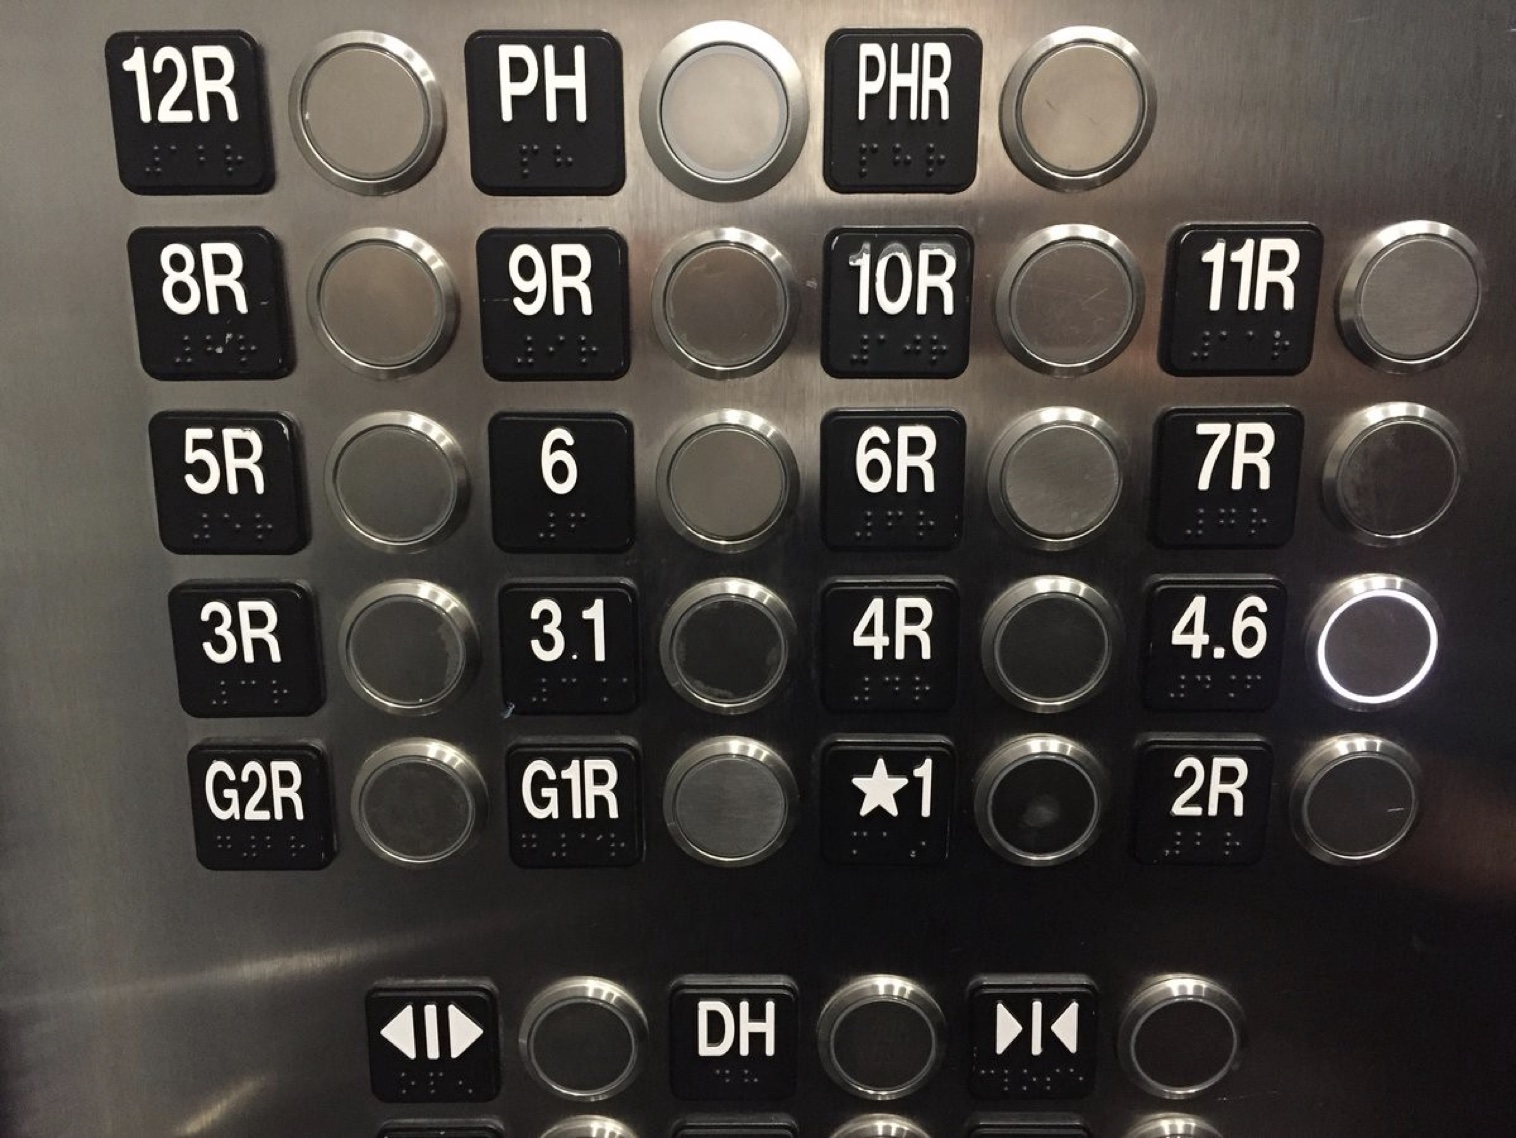
\includegraphics[width=0.3\linewidth]{controlpanel}
	\caption{The interface of the control panel has many fundamental design issues, and has room for improvement as presented in section}
	\label{fig:controlpanel}
\end{figure}

\subsection{Design changes to the elevator control panel:}

\begin{enumerate}
	\item Buttons/physical affordances could be raised a bit so as to give a good haptic feedback after it is clicked.
	\item Buttons could be arranged floor wise. Each row corresponds to a separate floor. It is common human tendency to look at buttons below if we are intending to traverse to lower floors and look for buttons on top, if we are intending to travel top floors.
	\item Logo of some floors - Eg: Parking, Gym, Roof, Basement instead of numbers.
	\item Labels should be placed on top of the buttons itself for better space utilization.
	\item A legend / key should be provided to understand the labelling for new visitors.
	\item A visual panel to understand what floor we’re traversing through. 
	\item Auditory feedback informing what button is pressed, where the elevator is headed.
	\item Physical display showing the progress of the elevator as it goes through each floor before reaching the destination.
	\item Control panel should have separate buttons in case of emergency with different colors and adhering to universal symbols for - HELP!, SOS ALARM!
	\end{enumerate}

\begin{figure}
	\centering
	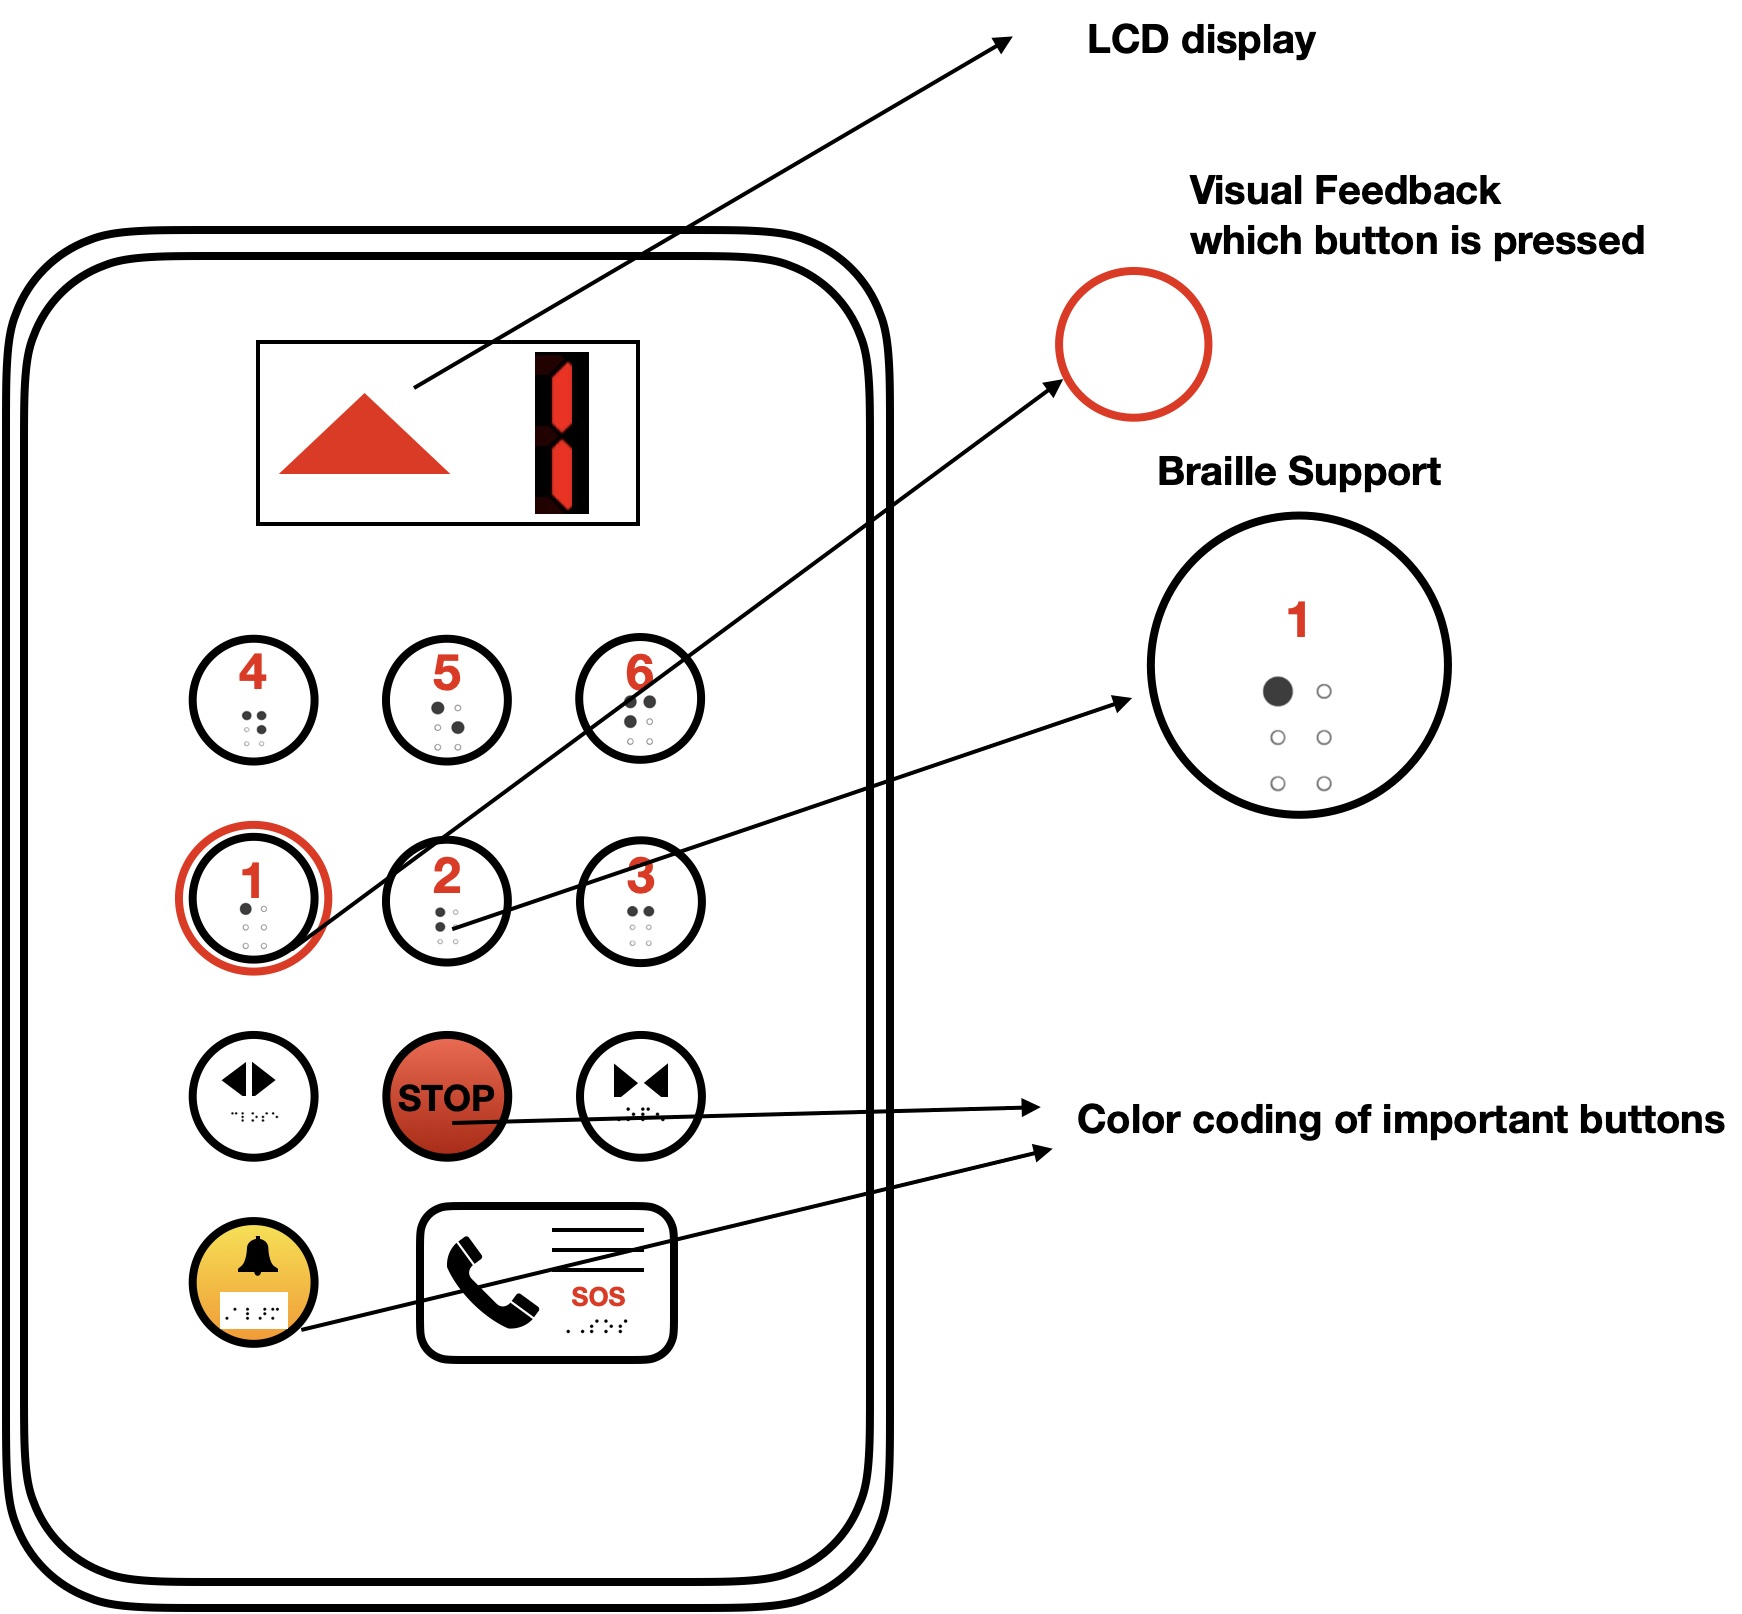
\includegraphics[width=0.3\linewidth]{revamp}
	\caption{We propose few modifications to the elevator control panel. The control panel has consistent rounded buttons, with visual feedback for floor information. The buttons also have braille script to accommodate people with disabilities.}
	\label{fig:revamp}
\end{figure}


\section{Bonus Question - Find two different user interfaces present in your environment and do the same analysis. Providing better designs is not mandatory this time, but would provide extra points. Provide pictures of these interfaces and a short summary of the possible interactions.}

In this section, we highlight two different user interfaces commonly encountered in everyday life and provide an analysis of the interfaces. We also suggest interesting changes that make the interface more holistic.

\subsection{Case Study - Apple Airpods}The Apple Airpods are bluetooth ear-phones with an unusual design. At the time they were released, the product was widely critiqued for looking like \emph{dental floss box} (See Figure \ref{fig:floss}).
\begin{enumerate}
		\item \textbf{Affordances} 
		\begin{itemize}
			\item At first glance, the physical affordance is not clear. Is the white box a dental floss or what?
		    \item If they are earphones how to use it (skip music? stop/play music)?
		    \item The affordance of the ear-phones is good, since it is apparent they are ear-phones and their utility is apparent.
			\end{itemize}
		\item \textbf{Visibility} 
		\begin{itemize}
	\item Because of the LED Indicators it is visible that the Airpods and the container are charged or not (and by the interaction with your smartphone)
	\item Have a bad visibility because you are not aware of what is going on, if the music is playing or not, if the volume is down
	\item Interacting with the Airpods is not possible without pairing with a smartphone.
	
		\end{itemize}
		
		\item \textbf{Feedback} 
		\begin{itemize}
\item Audio feedback is possible when the smartphone device is on and paired. 
\item When the device connects, the user will hear a specific sound. 
\item When the Airpods battery is low, you will hear a different sound; notifies on the phone device too.
\item The LED Indicator on the container will change color based on Airpods and deck battery.

		\end{itemize}
		\item \textbf{Mapping} 
		\begin{itemize}
\item The physical button is indistinguishable from the rest of the Airpod’s case making it difficult to discern the presence of the bluetooth's button and also its functionality of using it for pairing with the smartphone.
\item Individual ear-pieces are designed to be placed on the specific side of the ears. 


			
		\end{itemize}
		
		\item \textbf{Constraints} 
		\begin{itemize}
\item The product fits the user’s left or right ear specifically, less margin for error. 
\item The deck has a snug fit in the hand or in trouser pockets.
\item Logical constraints: There are strong constraints for charging the individual ear pieces. You’d have to put into the Airpod case for charging. The case itself cannot be used to charge something else.
\item Logical constraints: there no deck charge constraint, you have to use the apple wire but is lightning so you can put in which one direction do you prefer

		\end{itemize}
		
		\item \textbf{Consistency} 
		\begin{itemize}
			\item Possesses both Internal and External consistency.
			\item Behaves like every other wireless/bluetooth controlled earphones.
		\end{itemize}
		
		\item \textbf{Metaphors} 	
		\begin{itemize}
			\item No prevalent use of metaphors.
		\end{itemize}
		
		\item \textbf{Interaction Type}
		\begin{itemize}
\item Manipulation and Instructing.
\end{itemize}
\end{enumerate}


\begin{figure}
	\centering
	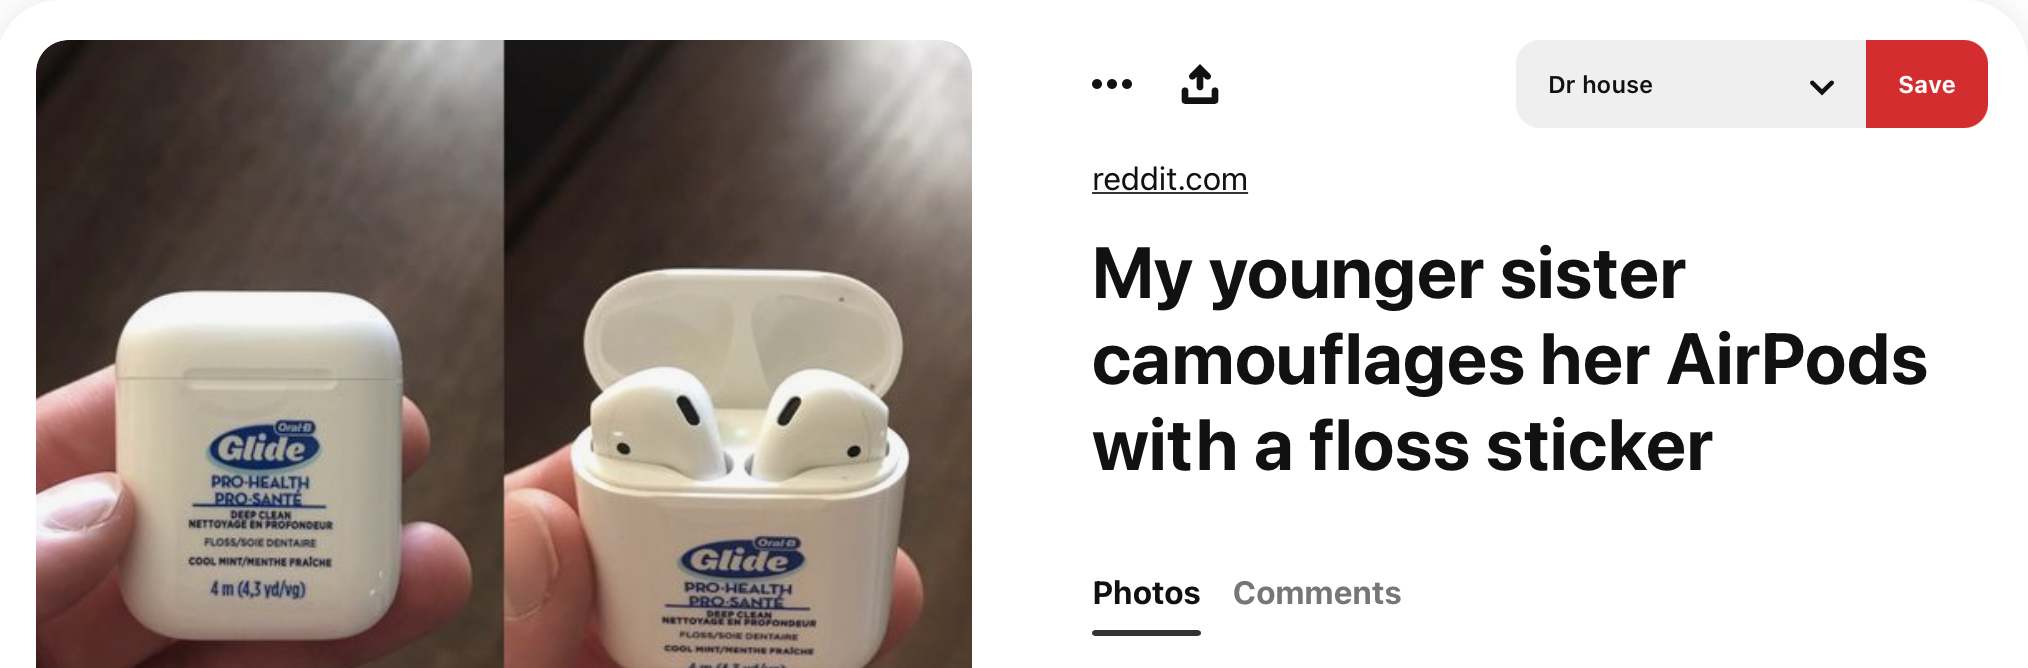
\includegraphics[width=0.5\linewidth]{floss}
	\caption{When the Airpods were first introduced, the design confused a lot of users. Some people even thought the box was a dental floss! Picture Credits :	\href{https://www.reddit.com/r/iphone/comments/bf5x3z/my_younger_sister_camouflages_her_airpods_with_a/?utm_source=ifttt}{Reddit}}
	\label{fig:floss}
\end{figure}



\subsubsection{Design changes to Apple Airpods}
In this section, we suggest few design changes to the Airpods, to make it more in-line with the foundations of interaction design.

\begin{enumerate}
	\item A small logo/icon on the Airpods' case to indicate they contain 'Ear-phones'.
	\item The Airpods houses a small button on the case, with no explanation of its functionality. We introduce a small icon that shows what the button can be used for.
	\item  The Airpods are designed to work in conjunction with the iPhone. However basic features such as the battery status of the Airpods case and the ear-phones can be provided with small LED like display as shown in the Figure \ref{fig:airpods}.
\end{enumerate}

\begin{figure}
	\centering
	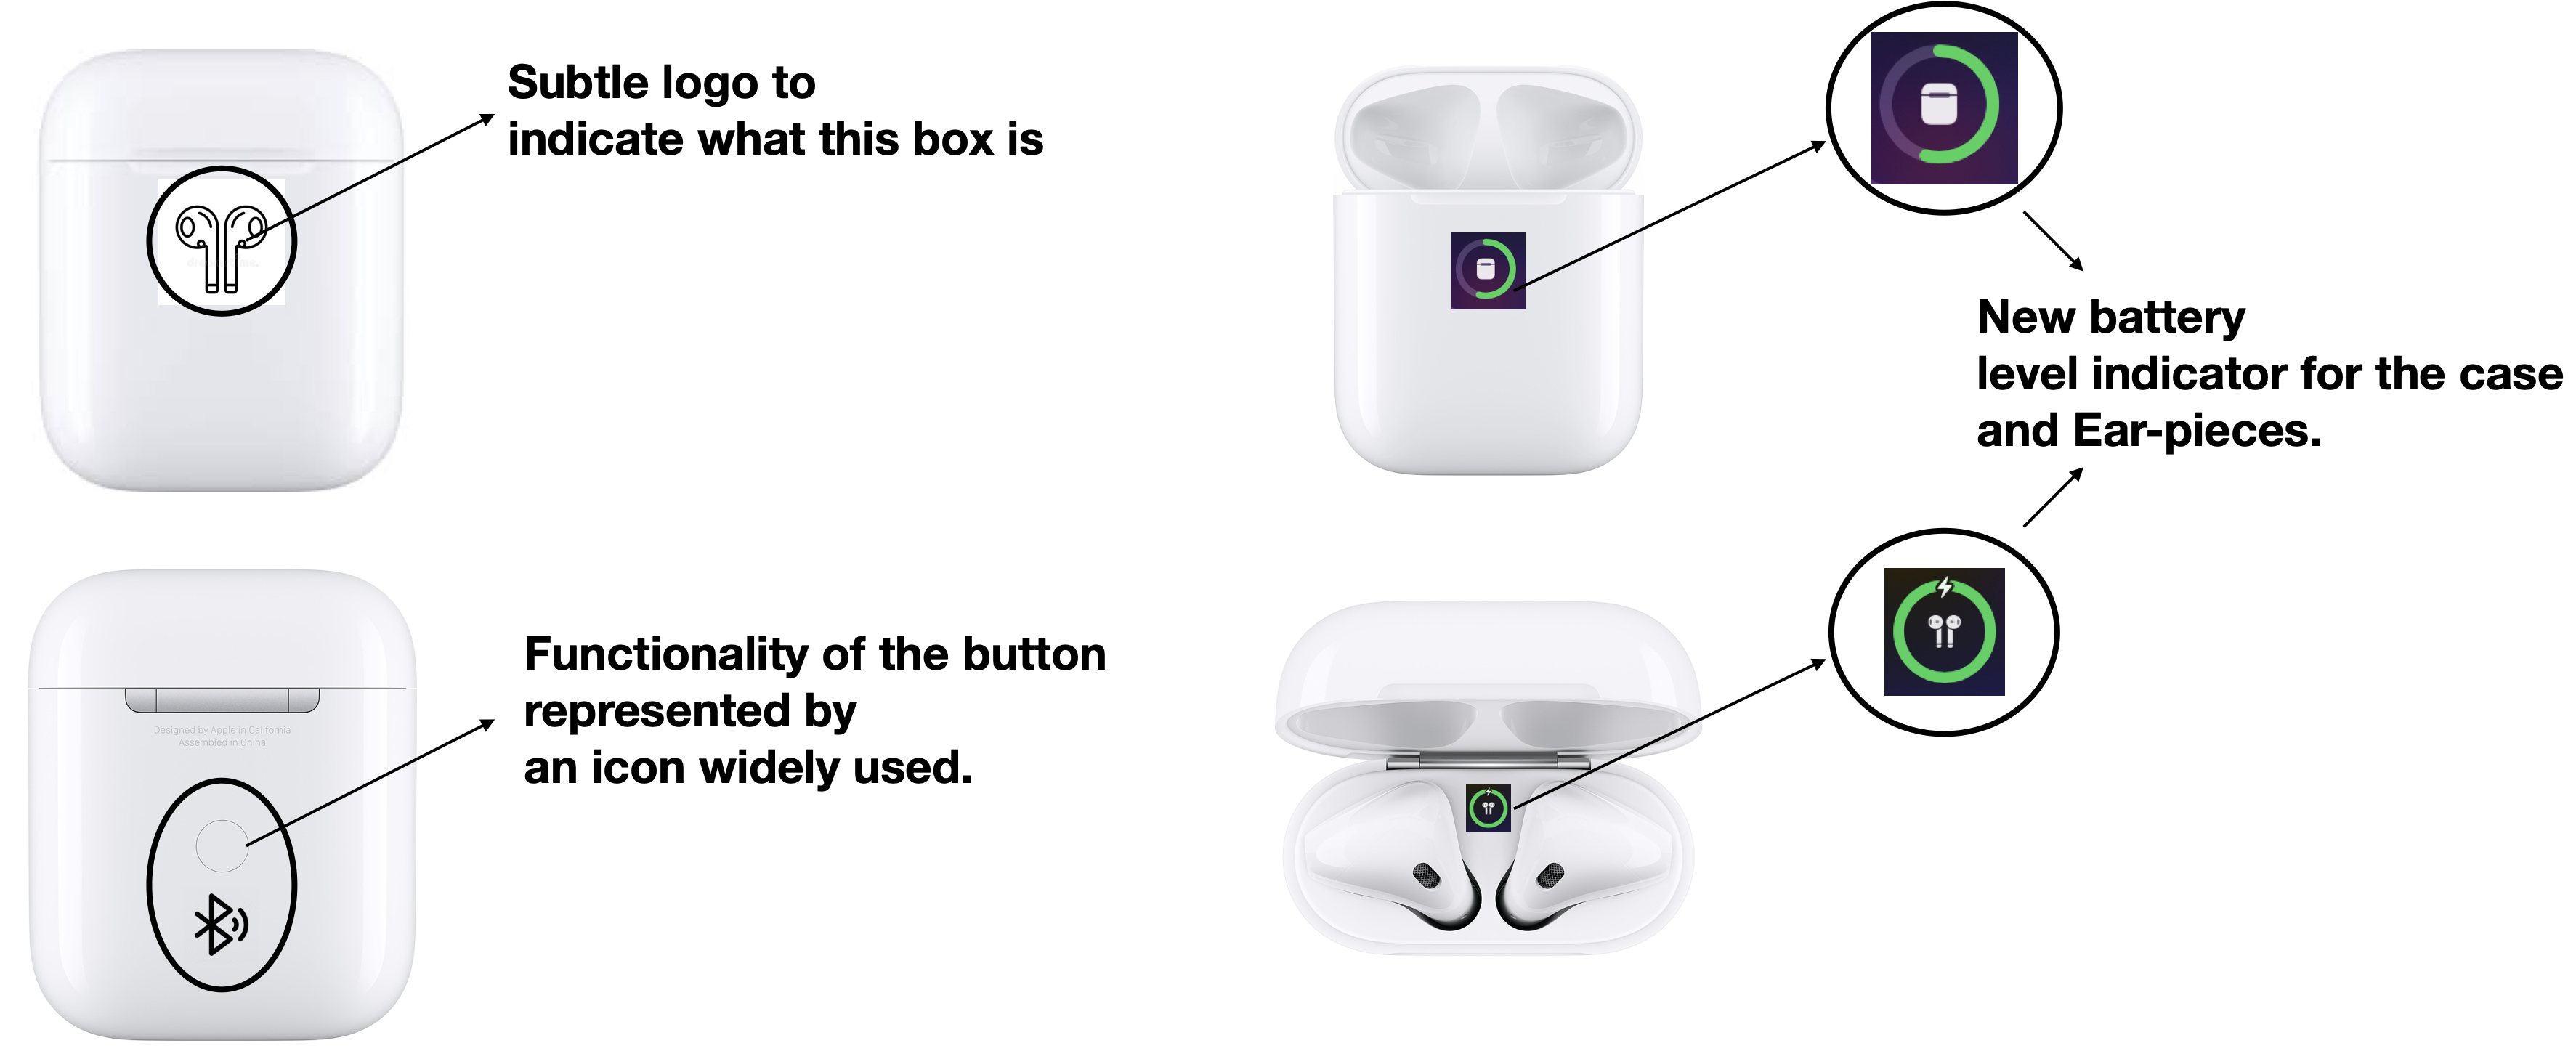
\includegraphics[width=0.7\linewidth]{airpods}
	\caption{In this exercise, we have provided interesting modifications to the existing Airpods design. We have provided with subtle logos/icons to indicate and highlight the different functionalities of the product.}
	\label{fig:airpods}
\end{figure}

\begin{figure}
	\centering
	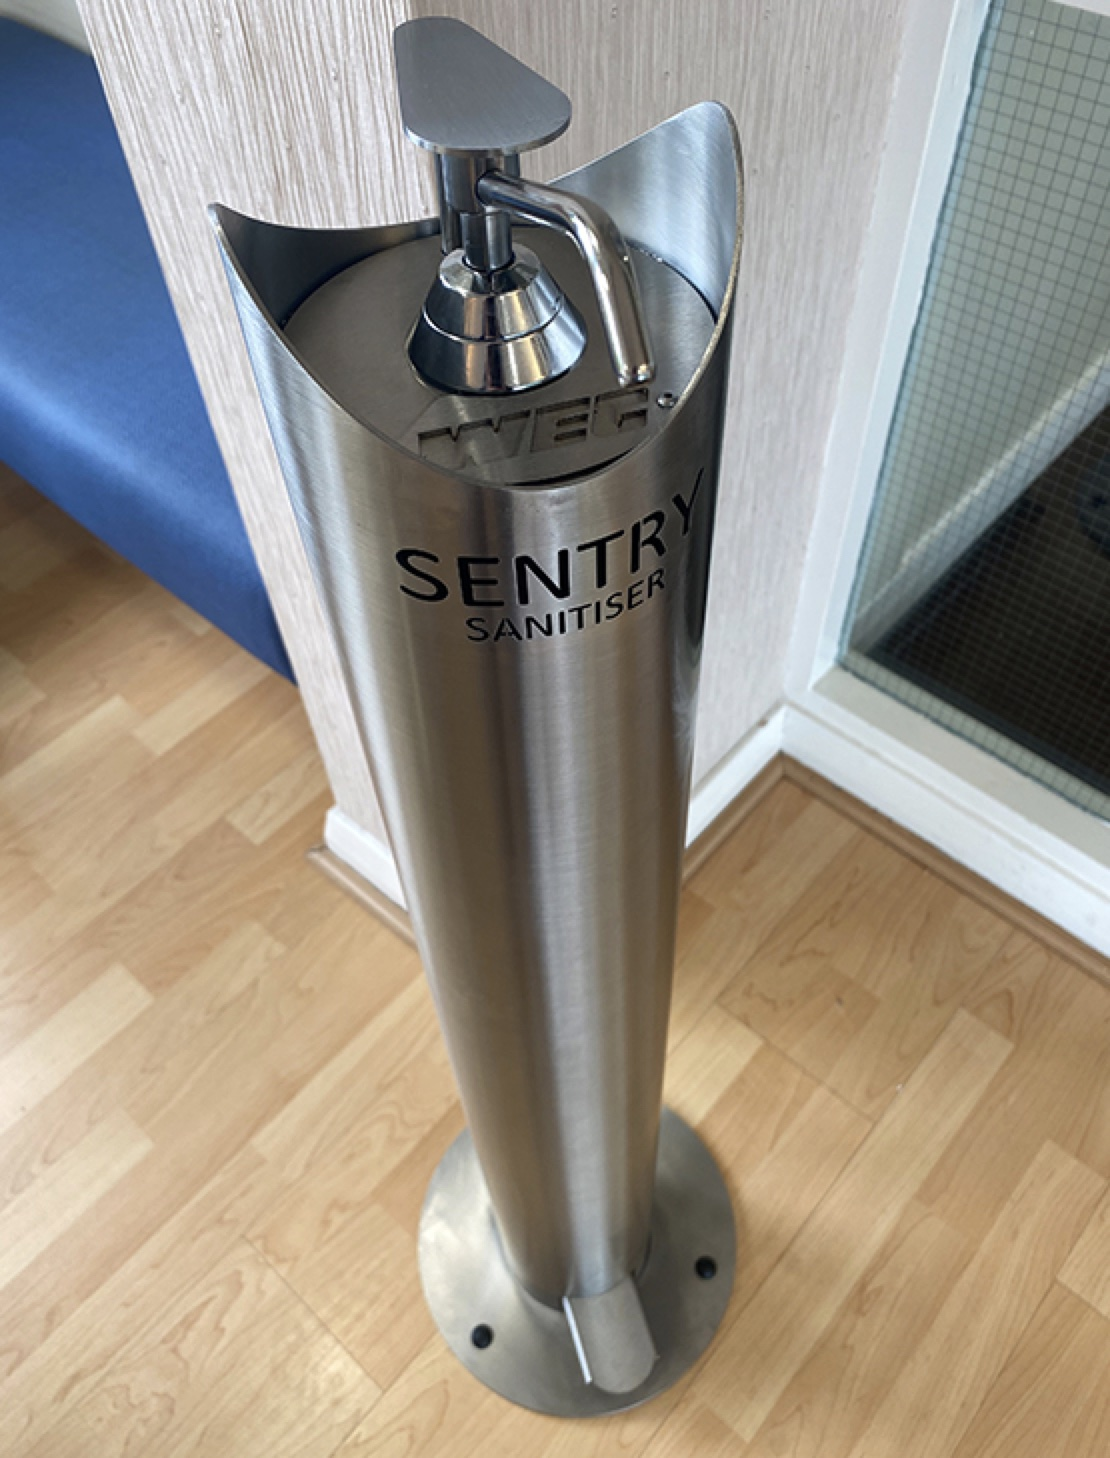
\includegraphics[width=0.3\linewidth]{san}
	\caption{Picture credit: \href{https://www.wec-group.com/hand-sanitiser-dispenser.html}{Foot operated Sanitizer}.}
	\label{fig:san}
\end{figure}
\subsection{Foot operated hand sanitizer} In this section, we study the interface of one of the most popular devices at recent times. A sanitizer dispensing machine, which can be operated with a pedal. See Figure \ref{fig:san}.

\begin{enumerate}
	\item \textbf{Affordances} 
	\begin{itemize}
	\item The current design suffers from poor physical affordance. It is not immediately clear whether the faucet for dispensing the disinfectant is the pedal or the one at the orifice.
	\end{itemize}
	\item \textbf{Visibility} 
	\begin{itemize}
		\item Looking at the dispenser, its clear the device has something to do with a liquid (water or something else). 
		\item However, its not obvious where the button is to dispense the liquid.		
	\end{itemize}
	
	\item \textbf{Feedback} 
	\begin{itemize}
		\item Once the operating procedure is figured out. The device provides good mechanical feedback, that is, you press the pedal, the liquid is dispensed, to indicate it is performing its core functionality.
		\item No feedback to indicate the level of disinfectant or if it should be re-filled.		
	\end{itemize}
	\item \textbf{Mapping} 
	\begin{itemize}
		\item Good spatial mapping and physical world analogy. Since the device is foot operated, the pedal resembles an artifact which evokes the response of pressing it.
		\item The pedal itself is not the highlight of the design.		
	\end{itemize}
	
	\item \textbf{Constraints} 
	\begin{itemize}
		\item The quantity of the disinfectant dispensed depends on the restricted movement of the pedal. The machine cannot dispense the liquid beyond the degree of freedom dictated by the pedal.	
	\end{itemize}
	
	\item \textbf{Consistency} 
	\begin{itemize}
\item Have a good internal consistency, it’s look like a device that dispenses a liquid, in this case a  disinfectant, and it acts like it.
\item The external consistency is pretty different because mostly of this structure are push by hand but that one is to push by foot

	\end{itemize}
	
	\item \textbf{Metaphors} 	
	\begin{itemize}
		\item The design physically resembles a water faucet. This allows the user to ascertain that the device should probably dispense some liquid.
	\end{itemize}
	
	\item \textbf{Interaction Type}
	\begin{itemize}
		\item Instructing interaction prevalent, you have only to press the button with your foot that is a repetitive action for the same task
	\end{itemize}
\end{enumerate}
\begin{figure}
	\centering
	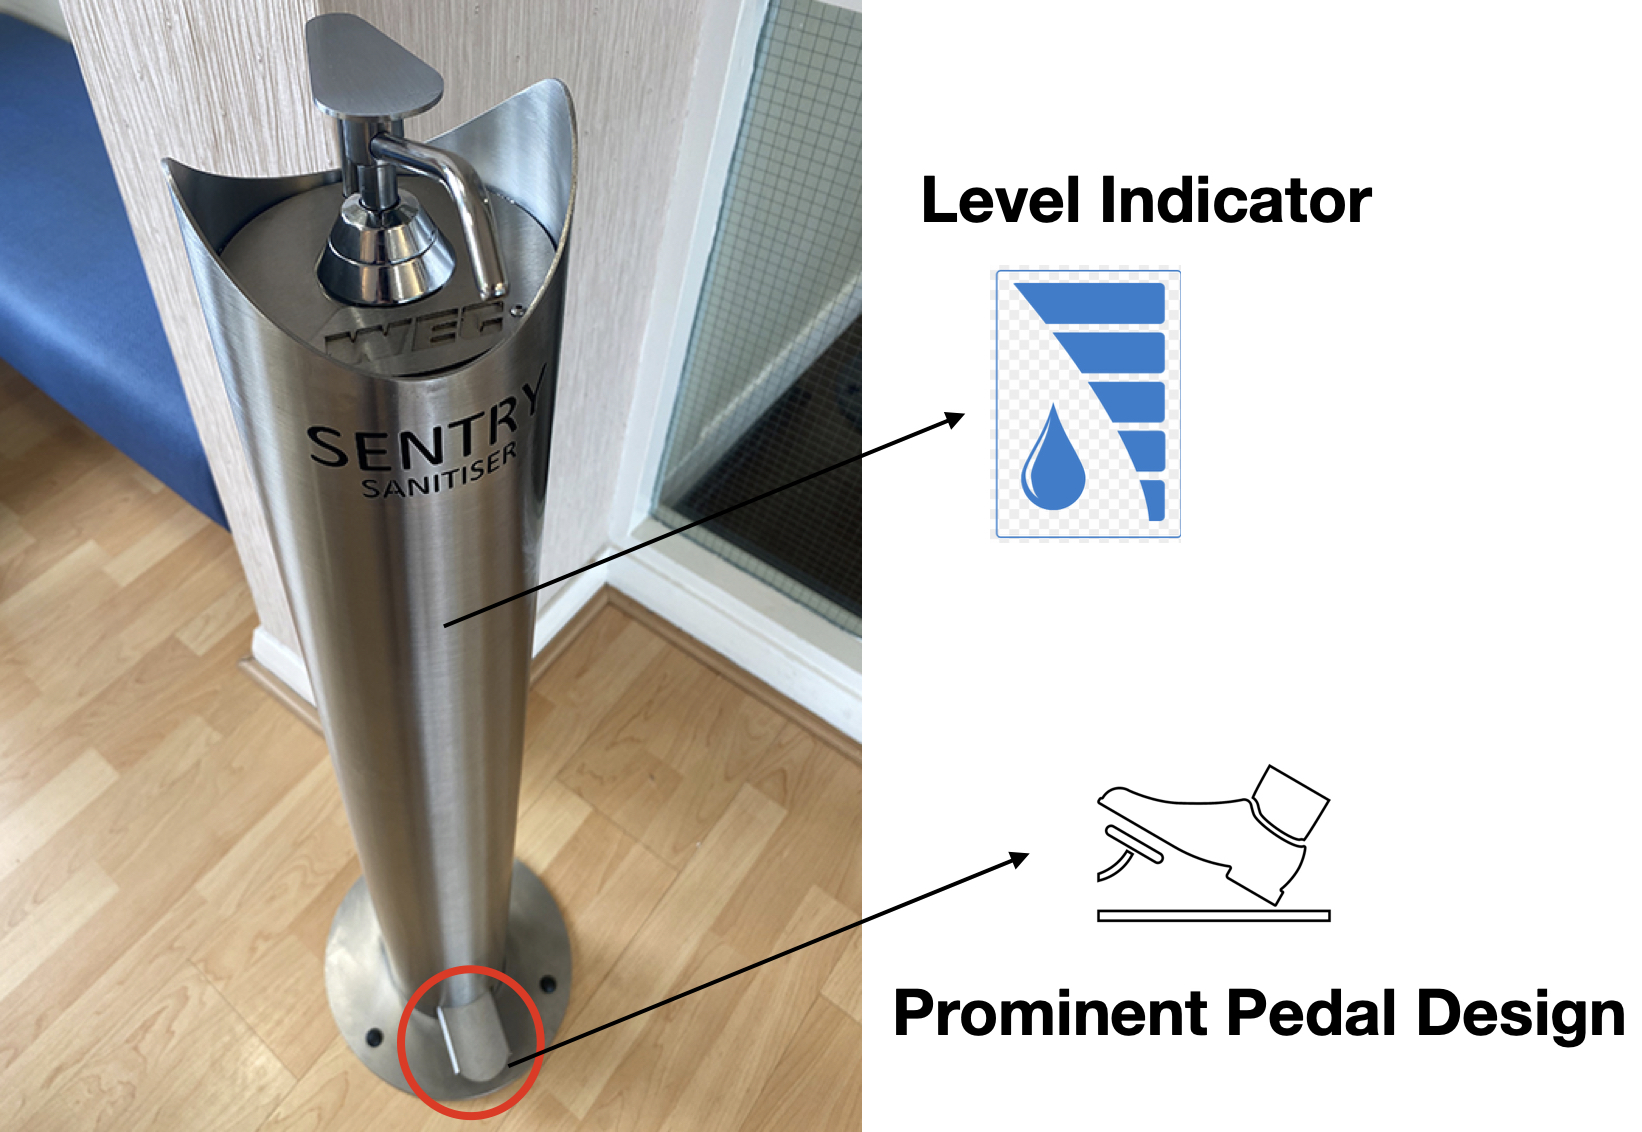
\includegraphics[width=0.3\linewidth]{san2}
	\caption{We propose few improvements to the existing foot operated sanitizer machine. Making the pedal more prominent and incorporating a feedback mechanism to alert for refill could potentially augment the usability of the device.}
	\label{fig:san2}
\end{figure}


\subsubsection{Design changes to the foot operated sanitizer}
\begin{enumerate}
	\item Allow to configure the dispensing angle of the disinfectant.
	\item A disinfectant level indicator to suggest refill.
	\item Making the pedal design more prominent.
\end{enumerate}


\begin{thebibliography}{widest entry}
\bibitem{book}
Jennifer Preece, Helen Sharp and Yvonne Rogers.
\textit{Interaction Design: Beyond Human-Computer Interaction, 4th Edition, Wiley, 2015}.	
\bibitem{airpodscase}
\href{https://bit.ly/2K8z2qN}{Airpods Logo}.
\bibitem{bt}
\href{https://bit.ly/32KegEc}{Bluetooth icon}.
\bibitem{case}
\href{www.apple.com}{Airpods case and Charging Logo}.
\bibitem{sink}
\href{https://www.wec-group.com/hand-sanitiser-dispenser.html}{Sanitizer Dispenser}.
\end{thebibliography}





\end{document}